\documentclass[a4paper,11pt]{article}
\usepackage[T1]{fontenc}
\usepackage[utf8]{inputenc}
\usepackage{lmodern}
\usepackage{textcomp}
\usepackage{amssymb}
\usepackage[margin=1.5cm]{geometry}
\usepackage{lscape}

\title{HICF1 -  Final Report v2}
\author{Dr. Susanne Weller}
\date{\today}

\usepackage{Sweave}
\begin{document}
\Sconcordance{concordance:HICF1_Finalreportv2.tex:HICF1_Finalreportv2.Rnw:%
1 13 1 1 0 5 1 1 39 1 30 1 4 35 0 1 2 1 1 1 46 1 4 43 0 1 2 2 1 1 4 43 %
0 1 2 14 1 1 18 1 12 1 3 2 1 1 4 79 1 1 33 6 1 1 35 1 5 31 0 1 2 165 1}


\maketitle

\section*{Univariate Analysis}


% Table created by stargazer v.5.1 by Marek Hlavac, Harvard University. E-mail: hlavac at fas.harvard.edu
% Date and time: Wed, Jul 30, 2014 - 16:47:03
\begin{table}[!htbp] \centering 
  \caption{Univariate Analysis against MRD outcome} 
  \label{} 
\tiny 
\begin{tabular}{@{\extracolsep{1p}} cccccccccc} 
\\[-1.8ex]\hline 
\hline \\[-1.8ex] 
 & p.value & uncorrected & corrected.p.value & corrected & MRDneg0 & MRDpos1 & MRDneg1 & sum & testused \\ 
\hline \\[-1.8ex] 
TP53\_ALL & $0.00004$ & \textasteriskcentered \textasteriskcentered \textasteriskcentered  & $0.001$ & \textasteriskcentered \textasteriskcentered \textasteriskcentered  & $105$ & $19$ & $2$ & $209$ & Fisher's Exact Test \\ 
TP53\_mut & $0.00001$ & \textasteriskcentered \textasteriskcentered \textasteriskcentered  & $0.0003$ & \textasteriskcentered \textasteriskcentered \textasteriskcentered  & $107$ & $15$ & $0$ & $209$ & Fisher's Exact Test \\ 
TP53\_bi & $0.009$ & \textasteriskcentered \textasteriskcentered  & $0.128$ & n.s. & $106$ & $9$ & $1$ & $209$ & Fisher's Exact Test \\ 
ATM\_ALL & $0.002$ & \textasteriskcentered \textasteriskcentered  & $0.033$ & \textasteriskcentered  & $83$ & $44$ & $24$ & $209$ & Fisher's Exact Test \\ 
ATM\_del & $0.0005$ & \textasteriskcentered \textasteriskcentered \textasteriskcentered  & $0.009$ & \textasteriskcentered \textasteriskcentered  & $98$ & $28$ & $9$ & $209$ & Fisher's Exact Test \\ 
BIRC3\_ALL & $0.094$ & trend & $0.850$ & n.s. & $94$ & $22$ & $13$ & $209$ & Fisher's Exact Test \\ 
BIRC3\_del & $0.002$ & \textasteriskcentered \textasteriskcentered  & $0.031$ & \textasteriskcentered  & $101$ & $21$ & $6$ & $209$ & Fisher's Exact Test \\ 
ATM\_bi & $0.002$ & \textasteriskcentered \textasteriskcentered  & $0.033$ & \textasteriskcentered  & $102$ & $19$ & $5$ & $209$ & Fisher's Exact Test \\ 
BIRC3\_bi & $0.360$ & n.s. & $1$ & n.s. & $106$ & $3$ & $1$ & $209$ & Fisher's Exact Test \\ 
ATM\_mono & $0.836$ & n.s. & $1$ & n.s. & $93$ & $12$ & $14$ & $209$ & Fisher's Exact Test \\ 
BIRC3\_mono & $0.066$ & trend & $0.723$ & n.s. & $100$ & $1$ & $7$ & $209$ & Fisher's Exact Test \\ 
NOTCH1\_mut & $0.069$ & trend & $0.723$ & n.s. & $88$ & $9$ & $19$ & $209$ & Fisher's Exact Test \\ 
SF3B1\_mut & $0.415$ & n.s. & $1$ & n.s. & $85$ & $26$ & $22$ & $209$ & Fisher's Exact Test \\ 
Trisomy\_12 & $0.002$ & \textasteriskcentered \textasteriskcentered  & $0.036$ & \textasteriskcentered  & $82$ & $8$ & $25$ & $209$ & Fisher's Exact Test \\ 
SAMHD1\_ALL & $0.054$ & trend & $0.657$ & n.s. & $105$ & $8$ & $2$ & $209$ & Fisher's Exact Test \\ 
Subclones & $0.050$ & trend & $0.657$ & n.s. & $$ & $$ & $$ & $$ & Wilcoxon Test \\ 
Total\_num\_CNAs & $0.483$ & n.s. & $1$ & n.s. & $$ & $$ & $$ & $$ & Wilcoxon Test \\ 
Binet & $0.770$ & n.s. & $1$ & n.s. & $72$ & $36$ & $35$ & $209$ & Fisher's Exact Test \\ 
age\_at\_randomisation & $0.100$ & trend & $0.850$ & n.s. & $$ & $$ & $$ & $$ & Wilcoxon Test \\ 
patient\_gender & $0.443$ & n.s. & $1$ & n.s. & $33$ & $76$ & $74$ & $209$ & Fisher's Exact Test \\ 
vh\_mutation\_status & $0.0003$ & \textasteriskcentered \textasteriskcentered \textasteriskcentered  & $0.006$ & \textasteriskcentered \textasteriskcentered  & $55$ & $60$ & $40$ & $181$ & Fisher's Exact Test \\ 
WBC & $0.013$ & \textasteriskcentered  & $0.179$ & n.s. & $$ & $$ & $$ & $$ & Wilcoxon Test \\ 
cd38 & $0.707$ & n.s. & $1$ & n.s. & $45$ & $40$ & $59$ & $147$ & Fisher's Exact Test \\ 
\hline \\[-1.8ex] 
\end{tabular} 
\end{table} 
\section*{Associations}
\begin{landscape}
% Table created by stargazer v.5.1 by Marek Hlavac, Harvard University. E-mail: hlavac at fas.harvard.edu
% Date and time: Wed, Jul 30, 2014 - 16:47:03
\begin{table}[!htbp] \centering 
  \caption{Uncorrected p-values for association between genetic lesions} 
  \label{} 
\tiny 
\begin{tabular}{@{\extracolsep{1p}} ccccccccccccccccccccccccccccccccc} 
\\[-1.8ex]\hline 
\hline \\[-1.8ex] 
 & variables & TP53\_ALL & TP53\_del & TP53\_cnLOH & TP53\_mut & ATM\_ALL & ATM\_mut & ATM\_del & ATM\_cnLOH & BIRC3\_ALL & BIRC3\_mut & BIRC3\_del & NOTCH1\_mut & SF3B1\_mut & X6q.\_del\_ALL & X13q\_ALL & Trisomy\_12 & Trisomy\_18 & Trisomy\_19 & XPO1\_gain & SAMHD1\_ALL & MYD88\_mut & MED12mutation & X8q\_ALL & Subclones & Total\_num\_CNAs & Binet & age\_at\_randomisation & patient\_gender & vh\_mutation\_status & WBC & cd38 \\ 
\hline \\[-1.8ex] 
1 & TP53\_ALL & $$ & $0$ & $0.001$ & $0$ & $0$ & $0.510$ & $0.571$ & $0.498$ & $1$ & $0.411$ & $0.343$ & $1$ & $0.593$ & $0.386$ & $0.444$ & $1$ & $0.627$ & $0.636$ & $0.432$ & $0.422$ & $0.101$ & $0.690$ & $0.083$ & $0.655$ & $0.073$ & $0.038$ & $0$ & $0.143$ & $1$ & $1$ & $0.202$ \\ 
2 & TP53\_del & $$ & $$ & $1$ & $0$ & $0$ & $0.274$ & $0.530$ & $0.429$ & $1$ & $1$ & $0.422$ & $1$ & $0.642$ & $0.634$ & $1$ & $1$ & $0.670$ & $1$ & $0.648$ & $0.181$ & $0.467$ & $0.825$ & $0.634$ & $1$ & $0.183$ & $0.412$ & $0.081$ & $0.417$ & $1$ & $1$ & $0.073$ \\ 
3 & TP53\_cnLOH & $$ & $$ & $$ & $0.005$ & $0.002$ & $1$ & $0.632$ & $0.505$ & $1$ & $1$ & $1$ & $1$ & $1$ & $1$ & $1$ & $0.209$ & $1$ & $1$ & $0.101$ & $0.596$ & $1$ & $0.169$ & $1$ & $0.091$ & $0.609$ & $1$ & $0.638$ & $1$ & $1$ & $1$ & $1$ \\ 
4 & TP53\_mut & $$ & $$ & $$ & $$ & $0$ & $0.173$ & $0.186$ & $0.275$ & $1$ & $0.631$ & $0.087$ & $0.642$ & $0.189$ & $0.181$ & $1$ & $1$ & $1$ & $1$ & $1$ & $1$ & $0.357$ & $0.875$ & $0.181$ & $0.377$ & $0.099$ & $0.125$ & $0.006$ & $0.083$ & $1$ & $1$ & $0.045$ \\ 
5 & ATM\_ALL & $$ & $$ & $$ & $$ & $$ & $0.642$ & $0.595$ & $0.527$ & $1$ & $0.505$ & $0.183$ & $1$ & $0.429$ & $0.416$ & $1$ & $0.560$ & $0.482$ & $1$ & $1$ & $0.386$ & $0.585$ & $1$ & $0.416$ & $0.536$ & $0.392$ & $0.276$ & $0.025$ & $0.181$ & $1$ & $1$ & $0.153$ \\ 
6 & ATM\_mut & $$ & $$ & $$ & $$ & $$ & $$ & $0$ & $0$ & $0.031$ & $0.001$ & $0$ & $0.373$ & $0$ & $0$ & $0.031$ & $0$ & $0$ & $0.593$ & $0.441$ & $0.548$ & $0.655$ & $0.803$ & $0.740$ & $0.855$ & $0.192$ & $0$ & $0.832$ & $0.045$ & $0.281$ & $0.186$ & $0.858$ \\ 
7 & ATM\_del & $$ & $$ & $$ & $$ & $$ & $$ & $$ & $0.003$ & $0.011$ & $0$ & $0.111$ & $0.197$ & $0.017$ & $0$ & $0.647$ & $0.058$ & $0$ & $0.530$ & $0.157$ & $0.584$ & $0.605$ & $0.516$ & $0.251$ & $0.918$ & $0.348$ & $0$ & $0.094$ & $0.051$ & $0.416$ & $0.272$ & $0.677$ \\ 
8 & ATM\_cnLOH & $$ & $$ & $$ & $$ & $$ & $$ & $$ & $$ & $1$ & $0.283$ & $0$ & $0.018$ & $0$ & $0$ & $0.002$ & $0$ & $0.002$ & $0.697$ & $0.829$ & $0.404$ & $0.342$ & $1$ & $0.345$ & $0.538$ & $0.189$ & $0.005$ & $0.384$ & $0.074$ & $0.632$ & $0.640$ & $0.200$ \\ 
9 & BIRC3\_ALL & $$ & $$ & $$ & $$ & $$ & $$ & $$ & $$ & $$ & $1$ & $1$ & $1$ & $1$ & $0$ & $1$ & $1$ & $1$ & $1$ & $1$ & $0.312$ & $1$ & $0.348$ & $0.432$ & $0.474$ & $1$ & $1$ & $0.192$ & $1$ & $1$ & $1$ & $1$ \\ 
10 & BIRC3\_mut & $$ & $$ & $$ & $$ & $$ & $$ & $$ & $$ & $$ & $$ & $0.277$ & $1$ & $0.413$ & $0.650$ & $1$ & $1$ & $0$ & $1$ & $1$ & $0.353$ & $1$ & $0.544$ & $0.393$ & $0.649$ & $0.065$ & $0.425$ & $0.183$ & $0.273$ & $1$ & $1$ & $1$ \\ 
11 & BIRC3\_del & $$ & $$ & $$ & $$ & $$ & $$ & $$ & $$ & $$ & $$ & $$ & $0$ & $0$ & $0$ & $0.002$ & $0$ & $0.003$ & $0$ & $0.662$ & $1$ & $0.743$ & $0.821$ & $0.338$ & $0.706$ & $0.507$ & $0.005$ & $0.180$ & $0.688$ & $0.266$ & $0.114$ & $0.195$ \\ 
12 & NOTCH1\_mut & $$ & $$ & $$ & $$ & $$ & $$ & $$ & $$ & $$ & $$ & $$ & $$ & $0.042$ & $1$ & $0$ & $1$ & $0.182$ & $0$ & $0.053$ & $1$ & $0.611$ & $0.858$ & $1$ & $1$ & $1$ & $0.284$ & $0.027$ & $0.034$ & $0.055$ & $0.010$ & $0.412$ \\ 
13 & SF3B1\_mut & $$ & $$ & $$ & $$ & $$ & $$ & $$ & $$ & $$ & $$ & $$ & $$ & $$ & $0$ & $0$ & $0$ & $0.017$ & $0.642$ & $0.449$ & $0.845$ & $0.713$ & $0.897$ & $0.273$ & $0.664$ & $0.439$ & $0.025$ & $0.611$ & $0.100$ & $1$ & $1$ & $0.380$ \\ 
14 & X6q.\_del\_ALL & $$ & $$ & $$ & $$ & $$ & $$ & $$ & $$ & $$ & $$ & $$ & $$ & $$ & $$ & $1$ & $0.416$ & $0.025$ & $1$ & $0.594$ & $0.216$ & $0.241$ & $0.496$ & $1$ & $0.445$ & $0.422$ & $0.037$ & $0.154$ & $0.025$ & $1$ & $1$ & $0.529$ \\ 
15 & X13q\_ALL & $$ & $$ & $$ & $$ & $$ & $$ & $$ & $$ & $$ & $$ & $$ & $$ & $$ & $$ & $$ & $1$ & $1$ & $1$ & $0.488$ & $1$ & $1$ & $1$ & $1$ & $1$ & $1$ & $1$ & $0.413$ & $1$ & $1$ & $1$ & $1$ \\ 
16 & Trisomy\_12 & $$ & $$ & $$ & $$ & $$ & $$ & $$ & $$ & $$ & $$ & $$ & $$ & $$ & $$ & $$ & $$ & $0.287$ & $1$ & $0.712$ & $0.564$ & $0.585$ & $1$ & $0.416$ & $0.536$ & $0.150$ & $0.276$ & $0.025$ & $0.731$ & $1$ & $1$ & $0.649$ \\ 
17 & Trisomy\_18 & $$ & $$ & $$ & $$ & $$ & $$ & $$ & $$ & $$ & $$ & $$ & $$ & $$ & $$ & $$ & $$ & $$ & $0.415$ & $0.252$ & $0.859$ & $1$ & $0.907$ & $0.206$ & $0.600$ & $0.602$ & $0.012$ & $0.356$ & $0.672$ & $1$ & $0.633$ & $0.177$ \\ 
18 & Trisomy\_19 & $$ & $$ & $$ & $$ & $$ & $$ & $$ & $$ & $$ & $$ & $$ & $$ & $$ & $$ & $$ & $$ & $$ & $$ & $0.047$ & $1$ & $0.467$ & $1$ & $1$ & $1$ & $1$ & $0.412$ & $0.081$ & $0.006$ & $0.027$ & $0.003$ & $1$ \\ 
19 & XPO1\_gain & $$ & $$ & $$ & $$ & $$ & $$ & $$ & $$ & $$ & $$ & $$ & $$ & $$ & $$ & $$ & $$ & $$ & $$ & $$ & $0.129$ & $0.728$ & $0.078$ & $0.279$ & $0.261$ & $0.458$ & $0.017$ & $0$ & $0.020$ & $0.553$ & $0.609$ & $1$ \\ 
20 & SAMHD1\_ALL & $$ & $$ & $$ & $$ & $$ & $$ & $$ & $$ & $$ & $$ & $$ & $$ & $$ & $$ & $$ & $$ & $$ & $$ & $$ & $$ & $0.160$ & $0.843$ & $0.537$ & $0.443$ & $0.145$ & $0.001$ & $0$ & $0.003$ & $1$ & $1$ & $1$ \\ 
21 & MYD88\_mut & $$ & $$ & $$ & $$ & $$ & $$ & $$ & $$ & $$ & $$ & $$ & $$ & $$ & $$ & $$ & $$ & $$ & $$ & $$ & $$ & $$ & $1$ & $1$ & $0.687$ & $1$ & $0.284$ & $1$ & $0.737$ & $1$ & $1$ & $1$ \\ 
22 & MED12mutation & $$ & $$ & $$ & $$ & $$ & $$ & $$ & $$ & $$ & $$ & $$ & $$ & $$ & $$ & $$ & $$ & $$ & $$ & $$ & $$ & $$ & $$ & $0.002$ & $0$ & $0$ & $0.001$ & $0$ & $0$ & $1$ & $1$ & $0.382$ \\ 
23 & X8q\_ALL & $$ & $$ & $$ & $$ & $$ & $$ & $$ & $$ & $$ & $$ & $$ & $$ & $$ & $$ & $$ & $$ & $$ & $$ & $$ & $$ & $$ & $$ & $$ & $0$ & $0.152$ & $0.001$ & $0$ & $0.139$ & $1$ & $1$ & $0.336$ \\ 
24 & Subclones & $$ & $$ & $$ & $$ & $$ & $$ & $$ & $$ & $$ & $$ & $$ & $$ & $$ & $$ & $$ & $$ & $$ & $$ & $$ & $$ & $$ & $$ & $$ & $$ & $0$ & $0.055$ & $0$ & $0.001$ & $0.744$ & $0.772$ & $0.622$ \\ 
25 & Total\_num\_CNAs & $$ & $$ & $$ & $$ & $$ & $$ & $$ & $$ & $$ & $$ & $$ & $$ & $$ & $$ & $$ & $$ & $$ & $$ & $$ & $$ & $$ & $$ & $$ & $$ & $$ & $0.100$ & $0.005$ & $0.003$ & $0.655$ & $0.420$ & $0.664$ \\ 
26 & Binet & $$ & $$ & $$ & $$ & $$ & $$ & $$ & $$ & $$ & $$ & $$ & $$ & $$ & $$ & $$ & $$ & $$ & $$ & $$ & $$ & $$ & $$ & $$ & $$ & $$ & $$ & $0$ & $0.008$ & $1$ & $1$ & $0.085$ \\ 
27 & age\_at\_randomisation & $$ & $$ & $$ & $$ & $$ & $$ & $$ & $$ & $$ & $$ & $$ & $$ & $$ & $$ & $$ & $$ & $$ & $$ & $$ & $$ & $$ & $$ & $$ & $$ & $$ & $$ & $$ & $0$ & $1$ & $0.283$ & $0.848$ \\ 
28 & patient\_gender & $$ & $$ & $$ & $$ & $$ & $$ & $$ & $$ & $$ & $$ & $$ & $$ & $$ & $$ & $$ & $$ & $$ & $$ & $$ & $$ & $$ & $$ & $$ & $$ & $$ & $$ & $$ & $$ & $0.016$ & $0.001$ & $0.057$ \\ 
29 & vh\_mutation\_status & $$ & $$ & $$ & $$ & $$ & $$ & $$ & $$ & $$ & $$ & $$ & $$ & $$ & $$ & $$ & $$ & $$ & $$ & $$ & $$ & $$ & $$ & $$ & $$ & $$ & $$ & $$ & $$ & $$ & $0$ & $1$ \\ 
30 & WBC & $$ & $$ & $$ & $$ & $$ & $$ & $$ & $$ & $$ & $$ & $$ & $$ & $$ & $$ & $$ & $$ & $$ & $$ & $$ & $$ & $$ & $$ & $$ & $$ & $$ & $$ & $$ & $$ & $$ & $$ & $1$ \\ 
31 & cd38 & $$ & $$ & $$ & $$ & $$ & $$ & $$ & $$ & $$ & $$ & $$ & $$ & $$ & $$ & $$ & $$ & $$ & $$ & $$ & $$ & $$ & $$ & $$ & $$ & $$ & $$ & $$ & $$ & $$ & $$ & $$ \\ 
\hline \\[-1.8ex] 
\end{tabular} 
\end{table} \end{landscape}

\begin{landscape}
% Table created by stargazer v.5.1 by Marek Hlavac, Harvard University. E-mail: hlavac at fas.harvard.edu
% Date and time: Wed, Jul 30, 2014 - 16:47:04
\begin{table}[!htbp] \centering 
  \caption{Corrected p-values for association between genetic lesions} 
  \label{} 
\tiny 
\begin{tabular}{@{\extracolsep{1p}} ccccccccccccccccccccccccccccccccc} 
\\[-1.8ex]\hline 
\hline \\[-1.8ex] 
 & variables & TP53\_ALL & TP53\_del & TP53\_cnLOH & TP53\_mut & ATM\_ALL & ATM\_mut & ATM\_del & ATM\_cnLOH & BIRC3\_ALL & BIRC3\_mut & BIRC3\_del & NOTCH1\_mut & SF3B1\_mut & X6q.\_del\_ALL & X13q\_ALL & Trisomy\_12 & Trisomy\_18 & Trisomy\_19 & XPO1\_gain & SAMHD1\_ALL & MYD88\_mut & MED12mutation & X8q\_ALL & Subclones & Total\_num\_CNAs & Binet & age\_at\_randomisation & patient\_gender & vh\_mutation\_status & WBC & cd38 \\ 
\hline \\[-1.8ex] 
1 & TP53\_ALL & $$ & $0$ & $0.558$ & $0$ & $0$ & $1$ & $1$ & $1$ & $1$ & $1$ & $1$ & $1$ & $1$ & $1$ & $1$ & $1$ & $1$ & $1$ & $1$ & $1$ & $1$ & $1$ & $1$ & $1$ & $1$ & $1$ & $0.136$ & $1$ & $1$ & $1$ & $1$ \\ 
2 & TP53\_del & $$ & $$ & $1$ & $0$ & $0$ & $1$ & $1$ & $1$ & $1$ & $1$ & $1$ & $1$ & $1$ & $1$ & $1$ & $1$ & $1$ & $1$ & $1$ & $1$ & $1$ & $1$ & $1$ & $1$ & $1$ & $1$ & $1$ & $1$ & $1$ & $1$ & $1$ \\ 
3 & TP53\_cnLOH & $$ & $$ & $$ & $1$ & $0.727$ & $1$ & $1$ & $1$ & $1$ & $1$ & $1$ & $1$ & $1$ & $1$ & $1$ & $1$ & $1$ & $1$ & $1$ & $1$ & $1$ & $1$ & $1$ & $1$ & $1$ & $1$ & $1$ & $1$ & $1$ & $1$ & $1$ \\ 
4 & TP53\_mut & $$ & $$ & $$ & $$ & $0$ & $1$ & $1$ & $1$ & $1$ & $1$ & $1$ & $1$ & $1$ & $1$ & $1$ & $1$ & $1$ & $1$ & $1$ & $1$ & $1$ & $1$ & $1$ & $1$ & $1$ & $1$ & $1$ & $1$ & $1$ & $1$ & $1$ \\ 
5 & ATM\_ALL & $$ & $$ & $$ & $$ & $$ & $1$ & $1$ & $1$ & $1$ & $1$ & $1$ & $1$ & $1$ & $1$ & $1$ & $1$ & $1$ & $1$ & $1$ & $1$ & $1$ & $1$ & $1$ & $1$ & $1$ & $1$ & $1$ & $1$ & $1$ & $1$ & $1$ \\ 
6 & ATM\_mut & $$ & $$ & $$ & $$ & $$ & $$ & $0$ & $0$ & $1$ & $0.470$ & $0.005$ & $1$ & $0$ & $0$ & $1$ & $0.189$ & $0$ & $1$ & $1$ & $1$ & $1$ & $1$ & $1$ & $1$ & $1$ & $0.004$ & $1$ & $1$ & $1$ & $1$ & $1$ \\ 
7 & ATM\_del & $$ & $$ & $$ & $$ & $$ & $$ & $$ & $1$ & $1$ & $0.042$ & $1$ & $1$ & $1$ & $0$ & $1$ & $1$ & $0$ & $1$ & $1$ & $1$ & $1$ & $1$ & $1$ & $1$ & $1$ & $0.094$ & $1$ & $1$ & $1$ & $1$ & $1$ \\ 
8 & ATM\_cnLOH & $$ & $$ & $$ & $$ & $$ & $$ & $$ & $$ & $1$ & $1$ & $0$ & $1$ & $0$ & $0$ & $0.837$ & $0$ & $0.949$ & $1$ & $1$ & $1$ & $1$ & $1$ & $1$ & $1$ & $1$ & $1$ & $1$ & $1$ & $1$ & $1$ & $1$ \\ 
9 & BIRC3\_ALL & $$ & $$ & $$ & $$ & $$ & $$ & $$ & $$ & $$ & $1$ & $1$ & $1$ & $1$ & $0.122$ & $1$ & $1$ & $1$ & $1$ & $1$ & $1$ & $1$ & $1$ & $1$ & $1$ & $1$ & $1$ & $1$ & $1$ & $1$ & $1$ & $1$ \\ 
10 & BIRC3\_mut & $$ & $$ & $$ & $$ & $$ & $$ & $$ & $$ & $$ & $$ & $1$ & $1$ & $1$ & $1$ & $1$ & $1$ & $0$ & $1$ & $1$ & $1$ & $1$ & $1$ & $1$ & $1$ & $1$ & $1$ & $1$ & $1$ & $1$ & $1$ & $1$ \\ 
11 & BIRC3\_del & $$ & $$ & $$ & $$ & $$ & $$ & $$ & $$ & $$ & $$ & $$ & $0$ & $0$ & $0.007$ & $0.683$ & $0.063$ & $1$ & $0.004$ & $1$ & $1$ & $1$ & $1$ & $1$ & $1$ & $1$ & $1$ & $1$ & $1$ & $1$ & $1$ & $1$ \\ 
12 & NOTCH1\_mut & $$ & $$ & $$ & $$ & $$ & $$ & $$ & $$ & $$ & $$ & $$ & $$ & $1$ & $1$ & $0.008$ & $1$ & $1$ & $0$ & $1$ & $1$ & $1$ & $1$ & $1$ & $1$ & $1$ & $1$ & $1$ & $1$ & $1$ & $1$ & $1$ \\ 
13 & SF3B1\_mut & $$ & $$ & $$ & $$ & $$ & $$ & $$ & $$ & $$ & $$ & $$ & $$ & $$ & $0.001$ & $0.196$ & $0.006$ & $1$ & $1$ & $1$ & $1$ & $1$ & $1$ & $1$ & $1$ & $1$ & $1$ & $1$ & $1$ & $1$ & $1$ & $1$ \\ 
14 & X6q.\_del\_ALL & $$ & $$ & $$ & $$ & $$ & $$ & $$ & $$ & $$ & $$ & $$ & $$ & $$ & $$ & $1$ & $1$ & $1$ & $1$ & $1$ & $1$ & $1$ & $1$ & $1$ & $1$ & $1$ & $1$ & $1$ & $1$ & $1$ & $1$ & $1$ \\ 
15 & X13q\_ALL & $$ & $$ & $$ & $$ & $$ & $$ & $$ & $$ & $$ & $$ & $$ & $$ & $$ & $$ & $$ & $1$ & $1$ & $1$ & $1$ & $1$ & $1$ & $1$ & $1$ & $1$ & $1$ & $1$ & $1$ & $1$ & $1$ & $1$ & $1$ \\ 
16 & Trisomy\_12 & $$ & $$ & $$ & $$ & $$ & $$ & $$ & $$ & $$ & $$ & $$ & $$ & $$ & $$ & $$ & $$ & $1$ & $1$ & $1$ & $1$ & $1$ & $1$ & $1$ & $1$ & $1$ & $1$ & $1$ & $1$ & $1$ & $1$ & $1$ \\ 
17 & Trisomy\_18 & $$ & $$ & $$ & $$ & $$ & $$ & $$ & $$ & $$ & $$ & $$ & $$ & $$ & $$ & $$ & $$ & $$ & $1$ & $1$ & $1$ & $1$ & $1$ & $1$ & $1$ & $1$ & $1$ & $1$ & $1$ & $1$ & $1$ & $1$ \\ 
18 & Trisomy\_19 & $$ & $$ & $$ & $$ & $$ & $$ & $$ & $$ & $$ & $$ & $$ & $$ & $$ & $$ & $$ & $$ & $$ & $$ & $1$ & $1$ & $1$ & $1$ & $1$ & $1$ & $1$ & $1$ & $1$ & $1$ & $1$ & $1$ & $1$ \\ 
19 & XPO1\_gain & $$ & $$ & $$ & $$ & $$ & $$ & $$ & $$ & $$ & $$ & $$ & $$ & $$ & $$ & $$ & $$ & $$ & $$ & $$ & $1$ & $1$ & $1$ & $1$ & $1$ & $1$ & $1$ & $0.042$ & $1$ & $1$ & $1$ & $1$ \\ 
20 & SAMHD1\_ALL & $$ & $$ & $$ & $$ & $$ & $$ & $$ & $$ & $$ & $$ & $$ & $$ & $$ & $$ & $$ & $$ & $$ & $$ & $$ & $$ & $1$ & $1$ & $1$ & $1$ & $1$ & $0.296$ & $0$ & $1$ & $1$ & $1$ & $1$ \\ 
21 & MYD88\_mut & $$ & $$ & $$ & $$ & $$ & $$ & $$ & $$ & $$ & $$ & $$ & $$ & $$ & $$ & $$ & $$ & $$ & $$ & $$ & $$ & $$ & $1$ & $1$ & $1$ & $1$ & $1$ & $1$ & $1$ & $1$ & $1$ & $1$ \\ 
22 & MED12mutation & $$ & $$ & $$ & $$ & $$ & $$ & $$ & $$ & $$ & $$ & $$ & $$ & $$ & $$ & $$ & $$ & $$ & $$ & $$ & $$ & $$ & $$ & $0.686$ & $0$ & $0.001$ & $0.219$ & $0$ & $0.027$ & $1$ & $1$ & $1$ \\ 
23 & X8q\_ALL & $$ & $$ & $$ & $$ & $$ & $$ & $$ & $$ & $$ & $$ & $$ & $$ & $$ & $$ & $$ & $$ & $$ & $$ & $$ & $$ & $$ & $$ & $$ & $0.009$ & $1$ & $0.237$ & $0.098$ & $1$ & $1$ & $1$ & $1$ \\ 
24 & Subclones & $$ & $$ & $$ & $$ & $$ & $$ & $$ & $$ & $$ & $$ & $$ & $$ & $$ & $$ & $$ & $$ & $$ & $$ & $$ & $$ & $$ & $$ & $$ & $$ & $0.005$ & $1$ & $0.040$ & $0.265$ & $1$ & $1$ & $1$ \\ 
25 & Total\_num\_CNAs & $$ & $$ & $$ & $$ & $$ & $$ & $$ & $$ & $$ & $$ & $$ & $$ & $$ & $$ & $$ & $$ & $$ & $$ & $$ & $$ & $$ & $$ & $$ & $$ & $$ & $1$ & $1$ & $1$ & $1$ & $1$ & $1$ \\ 
26 & Binet & $$ & $$ & $$ & $$ & $$ & $$ & $$ & $$ & $$ & $$ & $$ & $$ & $$ & $$ & $$ & $$ & $$ & $$ & $$ & $$ & $$ & $$ & $$ & $$ & $$ & $$ & $0$ & $1$ & $1$ & $1$ & $1$ \\ 
27 & age\_at\_randomisation & $$ & $$ & $$ & $$ & $$ & $$ & $$ & $$ & $$ & $$ & $$ & $$ & $$ & $$ & $$ & $$ & $$ & $$ & $$ & $$ & $$ & $$ & $$ & $$ & $$ & $$ & $$ & $0.006$ & $1$ & $1$ & $1$ \\ 
28 & patient\_gender & $$ & $$ & $$ & $$ & $$ & $$ & $$ & $$ & $$ & $$ & $$ & $$ & $$ & $$ & $$ & $$ & $$ & $$ & $$ & $$ & $$ & $$ & $$ & $$ & $$ & $$ & $$ & $$ & $1$ & $0.407$ & $1$ \\ 
29 & vh\_mutation\_status & $$ & $$ & $$ & $$ & $$ & $$ & $$ & $$ & $$ & $$ & $$ & $$ & $$ & $$ & $$ & $$ & $$ & $$ & $$ & $$ & $$ & $$ & $$ & $$ & $$ & $$ & $$ & $$ & $$ & $0.001$ & $1$ \\ 
30 & WBC & $$ & $$ & $$ & $$ & $$ & $$ & $$ & $$ & $$ & $$ & $$ & $$ & $$ & $$ & $$ & $$ & $$ & $$ & $$ & $$ & $$ & $$ & $$ & $$ & $$ & $$ & $$ & $$ & $$ & $$ & $1$ \\ 
31 & cd38 & $$ & $$ & $$ & $$ & $$ & $$ & $$ & $$ & $$ & $$ & $$ & $$ & $$ & $$ & $$ & $$ & $$ & $$ & $$ & $$ & $$ & $$ & $$ & $$ & $$ & $$ & $$ & $$ & $$ & $$ & $$ \\ 
\hline \\[-1.8ex] 
\end{tabular} 
\end{table} \end{landscape}
Odds ratios and p-values for association between genes are represented in this heat map. Note that blue is mutually exclusive, red is associated. Also, the colour key is not symmetrical, colours used:
\begin{itemize}
  \item -3 -> oddsratio<0.1 
  \item -2 -> oddsratio>=0.1 & oddsratio < 0.2
  \item -1 -> oddsratio>=0.2 & oddsratio < 0.4
  \item  0 -> oddsratio>=0.4 & oddsratio < 0.6
  \item  1 -> oddsratio>=0.6 & oddsratio < 0.8
  \item  2 -> oddsratio>=1 & oddsratio < 3
  \item  3 -> oddsratio>=3 & oddsratio < 10
  \item  4 -> oddsratio>=10 & oddsratio < 15
  \item  5 -> oddsratio>=15 & oddsratio < 20
  \item  6 -> oddsratio>20
\end{itemize}\\


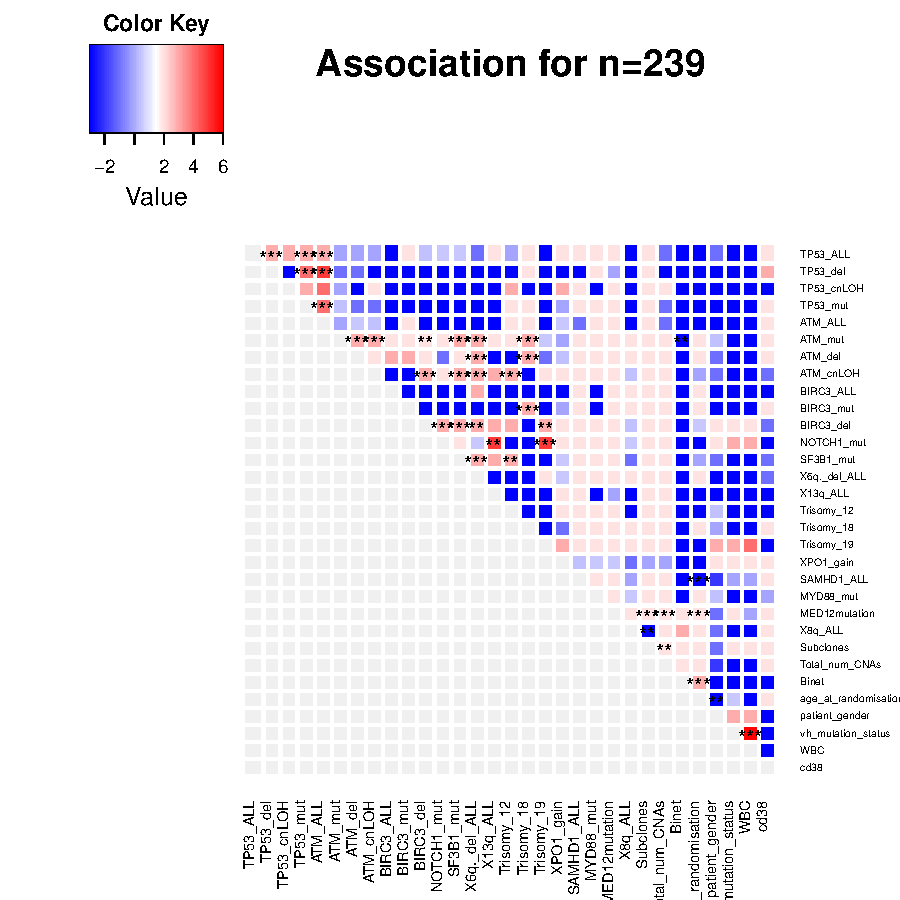
\includegraphics{HICF1_Finalreportv2-008}
\section*{Model building - from here, only 209 data points will be used}
% \section*{Association on model data}
% This was calculated to see if there are Colinearities that have to be taken into account for the modelling. There are fewer associations than in the 239 data set. 
% 
% <<Association on model data, echo=FALSE, eval=TRUE>>=
% source("/home/andreas/suska/work/01_HICF1/HICF1_sub1/trunk/HICF1_v6/Association.R")
% #produce a new data frame that contains variable names as first column
% #This makes the first column a list of all the variables used
% model.ass.pvalues <- colnames(model.genclinv6)
% model.ass.pvalues <- as.data.frame(model.ass.pvalues)
% names(model.ass.pvalues)[names(model.ass.pvalues)=="model.ass.pvalues"] <- "variables"
% #This just produces a list of all the variables used to go through in the for loops
% variables <- colnames(model.genclinv6)
% for (i in 1:52){
% model.ass.pvalues[variables[i]] <- NA
% }
% model.genclinv6$Subclones <- as.numeric(model.genclinv6$Subclones)
% model.genclinv6$Total_num_CNAs <- as.numeric(model.genclinv6$Total_num_CNAs)
% model.genclinv6$age_at_randomisation <- as.numeric(model.genclinv6$age_at_randomisation)
% for (i in 1:52){
%   for (j in 1:52){
%   model.ass.pvalues[i, j+1] <- association.pvalue(i, j) 
% }
% }
% 
% 
% model.ass.pvalues[,c(2:53)] <- lapply(model.ass.pvalues[,c(2:53)], as.numeric)
% 
% model.ass.pvalues.corrected <- as.matrix(model.ass.pvalues[, c(2:53)]) 
% model.ass.pvalues.corrected <- round(p.adjust(model.ass.pvalues.corrected, method="holm"), digits=3)
% model.ass.pvalues.corrected <- split(model.ass.pvalues.corrected, ceiling(seq_along(model.ass.pvalues.corrected)/length(model.ass.pvalues[[1]])))
% 
% model.ass.pvalues[,c(2:53)] <- round(model.ass.pvalues[,c(2:53)], digits=3)
% model.ass.pvalues.corrected <- as.data.frame(model.ass.pvalues.corrected)
% colnames(model.ass.pvalues.corrected) <- variables
% model.ass.pvalues.corrected <- cbind(variables, model.ass.pvalues.corrected)
% 
% # write.csv(model.ass.pvalues, file="/home/andreas/suska/work/01_HICF1/HICF1_sub1/trunk/HICF1_v6/Associationpvalues_model.csv", sep="\t")
% # write.csv(model.ass.pvalues.corrected, file="/home/andreas/suska/work/01_HICF1/HICF1_sub1/trunk/HICF1_v6/Associationpvalues_model_corrected.csv", sep="\t")
% 
% @
% 
% <<oddssratio, echo=FALSE, eval=TRUE>>=
% source("oddsratio.R")
% #This makes an empty data frame with the first line the list of variables used:
% model.ass.oddsratios <- colnames(model.genclinv6)
% model.ass.oddsratios <- as.data.frame(model.ass.oddsratios)
% names(model.ass.oddsratios)[names(model.ass.oddsratios)=="model.ass.oddsratios"] <- "variables"
% for (i in 1:52){
% model.ass.oddsratios[variables[i]] <- NA
% }
% 
% for (i in 1:52){
%   source("oddsratioscale.R")
%   for (j in 1:52){
%   model.ass.oddsratios[i, j+1] <- oddsratioscale(i, j) 
% }
% }
% @
% \begin{landscape}
% <<echo=FALSE, results=tex>>=
% #RESULT TABLE in a nice format!
% library(stargazer)
% stargazer(model.ass.pvalues.corrected, summary=FALSE, title="Corrected p-values for association between genetic lesions, n=209", font.size="tiny", column.sep.width="0p")
% @
% \end{landscape}
% <<fig=TRUE, echo=FALSE, eval=TRUE>>=
% # Set variables to row.names
% row.names(model.ass.oddsratios) <- model.ass.oddsratios$variables
% model.ass.oddsratios$variables <- NULL
% 
% #Produce matrix indicating significance
% source("significancelevels.R")
% sigstars <- apply(model.ass.pvalues.corrected[2:53], c(1,2), significancelevels) 
% 
% 
% library("gplots")
% heatmap.2((as.matrix(model.ass.oddsratios, rownames.force=TRUE)), col=bluered(75), scale="none", na.rm=TRUE, key=TRUE, symkey=FALSE, density.info="none", trace="none", cexRow=0.5, xlab="", ylab="", Rowv=FALSE, Colv=FALSE, cexCol = 0.7, sepwidth=c(0.1,0.1), sepcolor="white", rowsep=c(1:56), colsep=c(1:56), na.color="gray94", cellnote=sigstars, notecol="black", main="Model data, n=209")
% @

\section*{Logistic regression model}
\subsection*{Simple logistic regression models}
For these models, I used the variables that turned out significant in the univariate analysis (model 1-4 in table 5). This is a commonly used procedure, but it can mean that I selected variables that are highly colinear (or co-occuring), TP53 variables for example.
\subsection*{Summarized Model}
For these models, I summarized the data even more:
\begin{itemize}
  \item all trisomies are grouped together
  \item for each lesion, I used the broadest variable
\end{itemize}

%\begin{landscape}
% Table created by stargazer v.5.1 by Marek Hlavac, Harvard University. E-mail: hlavac at fas.harvard.edu
% Date and time: Wed, Jul 30, 2014 - 16:47:06
\begin{table}[!htbp] \centering 
  \caption{Multiple log regression, n=209} 
  \label{} 
\tiny 
\begin{tabular}{@{\extracolsep{5pt}}lcc} 
\\[-1.8ex]\hline 
\hline \\[-1.8ex] 
 & \multicolumn{2}{c}{\textit{Dependent variable:}} \\ 
\cline{2-3} 
\\[-1.8ex] & \multicolumn{2}{c}{MRD} \\ 
 & genetic 1 & genetic2 \\ 
\hline \\[-1.8ex] 
 TP53\_ALL1 & 2.51$^{***}$ (0.78) & 2.67$^{***}$ (0.78) \\ 
  ATM\_bi1 & 1.68$^{***}$ (0.56) &  \\ 
  BIRC3\_mono1 & $-$2.15$^{*}$ (1.27) &  \\ 
  ATM\_ALL1 &  & 0.99$^{***}$ (0.33) \\ 
  Trisomy\_121 & $-$0.76 (0.48) & $-$0.82 (0.52) \\ 
  NOTCH1\_mut1 & $-$0.61 (0.52) & $-$0.67 (0.53) \\ 
  SAMHD1\_ALL1 & 2.01$^{**}$ (0.89) & 1.63$^{**}$ (0.83) \\ 
  SF3B1\_mut1 &  & $-$0.16 (0.44) \\ 
  X13q\_Rossi1 & $-$0.30 (0.36) & $-$0.20 (0.41) \\ 
  Constant & $-$0.17 (0.25) & $-$0.35 (0.35) \\ 
 \hline \\[-1.8ex] 
Observations & 209 & 209 \\ 
Log Likelihood & $-$121.23 & $-$123.45 \\ 
Akaike Inf. Crit. & 258.46 & 262.89 \\ 
\hline 
\hline \\[-1.8ex] 
\textit{Note:}  & \multicolumn{2}{l}{$^{*}$p$<$0.1; $^{**}$p$<$0.05; $^{***}$p$<$0.01} \\ 
\end{tabular} 
\end{table} %\end{landscape}
% \subsection*{Discussion of different models}
% You can see that the model gets better, the simpler it is. It basically makes no sense at all to put everything we have into a regression model, it is better to use the broadest defined variables (Have to discuss this with Chris though). One good thing with the model that uses only genetic data is that it is as good as the model that includes vh mutation status. It is not really better, but apparently, vh mutation status is a measure that is hard to obtain, and not very reliable. We could argue that genetic testing can almost replace vh mutation status as a predictor for MRD. To harden this argument, I calculated the missclassification error for both models and they are almost identical, yet we have more unclassified when using the vh mutation status.

% \subsection*{Missclassification Error}
% <<Missclassification Error, echo=FALSE, eval=TRUE>>=
% missclasserror<- data.frame(matrix(NA, nrow = 2, ncol = 7))
% colnames(missclasserror) <- c("model", "true_MRD_neg","correct_MRD_neg","false_MRD_neg", "true_MRD_pos", "correct_MRD_pos", "false_MRD_pos") 
% missclasserror$model <- c("sum_genetic", "sum_vhmut")
% missclasserror$true_MRD_neg <- c(summary(model.genclinv6$MRD)[1], summary(model.genclinv6.genclin$MRD)[1])
% missclasserror$true_MRD_pos <- c(summary(model.genclinv6$MRD)[2], summary(model.genclinv6.genclin$MRD)[2])
% missclasserror$correct_MRD_neg <- c(table(model.genclinv6$MRD, model.genclinv6$model.gen.class)[1], table(model.genclinv6.genclin$MRD, model.genclinv6.genclin$model.genclin.class)[1])
% missclasserror$correct_MRD_pos <- c(table(model.genclinv6$MRD, model.genclinv6$model.gen.class)[4], table(model.genclinv6.genclin$MRD, model.genclinv6.genclin$model.genclin.class)[4])
% missclasserror$false_MRD_neg <- c(table(model.genclinv6$MRD, model.genclinv6$model.gen.class)[2], table(model.genclinv6.genclin$MRD, model.genclinv6.genclin$model.genclin.class)[2])
% missclasserror$false_MRD_pos <- c(table(model.genclinv6$MRD, model.genclinv6$model.gen.class)[3], table(model.genclinv6.genclin$MRD, model.genclinv6.genclin$model.genclin.class)[3])
% missclasserror$missclasserror <- (missclasserror$false_MRD_neg+missclasserror$false_MRD_pos)/(missclasserror$true_MRD_neg+missclasserror$true_MRD_pos)
% missclasserror$unclassified <- c(0, 29)
% @
% 
% <<echo=FALSE, results=tex>>=
% #RESULT TABLE in a nice format!
% library(stargazer)
% 
% stargazer(missclasserror, summary=FALSE, title="Missclassification for summarized models", font.size="tiny", single.row=TRUE,column.sep.width="1p")
% @

% # <<echo=FALSE, results=tex>>=
% # library(xtable)
% # glm <- xtable(fit.sum.gen)
% # print(glm)
% # 
% # @
% # 
% # % \subsection*{Logistic regression with Ridge}
% <<Ridge logistic regression, echo=FALSE, eval=TRUE>>=
% library(glmnet)
% x=data.matrix(genclinMRD[,c(1:48, 54, 55, 56)])
% y=genclinMRD$MRD
% ridge.model <- glmnet(x, y, family="binomial", alpha=0)
% ridge.model
% plot(ridge.model)
% summary(ridge.model)
% coef(ridge.model)
% #Crossvalidate to find optimal lambda:
% set.seed(1712)
% cv.ridge= cv.glmnet(x, y, alpha=0, family="binomial")
% plot(cv.ridge)
% bestlambda=cv.ridge$lambda.min
% bestlambda
% 
% #built model with optimal lambda using the predict function to look at the coefficients
% optimized.ridge.model <- predict(ridge.model, s=bestlambda, type="coefficient")
% optimized.ridge.model <- as.data.frame(as.matrix(optimized.ridge.model))
% colnames(optimized.ridge.model)[1]<- "coefficient_ridge"
% optimized.ridge.model$variables <- row.names(optimized.ridge.model)
% row.names(optimized.ridge.model) <- NULL
% 
% 
% @
% 
% \subsection*{Logistic regression with Lasso}
% <<Lasso logistic regression, echo=FALSE, eval=TRUE>>=
% library(glmnet)
% x=data.matrix(genclinMRD[,c(1:48, 54, 55, 56)])
% genclinMRD[51]
% y=as.numeric(genclinMRD$MRD)
% lasso.model <- glmnet(x, y, family="binomial", alpha=1)
% lasso.model
% plot(lasso.model)
% summary(lasso.model)
% coef(lasso.model)
% #Crossvalidate to find optimal lambda:
% set.seed(1712)
% cv.lasso= cv.glmnet(x, y, alpha=1, family="binomial")
% plot(cv.lasso)
% bestlambda=cv.lasso$lambda.min
% bestlambda
% 
% optimized.lasso.model <- predict(lasso.model, s=bestlambda, type="coefficient")
% optimized.lasso.model <- as.data.frame(as.matrix(optimized.lasso.model))
% colnames(optimized.lasso.model)[1]<- "coefficient_lasso"
% optimized.lasso.model$variables <- row.names(optimized.lasso.model)
% row.names(optimized.lasso.model) <- NULL
% @
% 
% \subsection*{Compare Lasso and Ridge Regression Coefficients}
% <<fig=TRUE, eval=TRUE, echo=FALSE>>=
% coefficients <- cbind(optimized.lasso.model, optimized.ridge.model)
% coefficients <- coefficients[2:52, ]
% library(ggplot2)
% ggplot()+geom_point(data=coefficients, aes(x=coefficient_lasso, y=coefficient_ridge))+
% geom_text(data=coefficients, aes(x=coefficient_lasso, y=coefficient_ridge, label = variables), vjust = 0.7, hjust = 1, size=3, col="darkblue")+
%   xlim(-1, 2)+
%   geom_hline(yintercept=0, alpha=0.5)+
%   geom_hline(yintercept=c(-0.1, 0.1), col="darkred", alpha=0.5, linetype="dashed")+
%   geom_vline(xintercept=0, alpha=0.5)
% @
% \subsection*{Find the best model with only important parameters (includes cutoff for ridge regression)}
% <<Model with results from lasso and ridge, echo=FALSE, eval=TRUE>>=
% variables_ridge_lasso_selected <- subset(coefficients, coefficient_lasso !=0)#& abs(coefficients$coefficient_ridge) > 0.4) 
% genclin_ridge_lasso_selected <- genclinMRD[,colnames(genclinMRD)%in%variables_ridge_lasso_selected$variables] 
% genclin_ridge_lasso_selected$MRD <- genclinMRD$MRD
% 
% system.time(best.subset.from.lasso <- bestglm(genclin_ridge_lasso_selected, family=binomial))
% best.subset.from.lasso
% fit_ridge_lasso_selected <- glm(MRD ~ ., family=binomial(logit), data=genclin_ridge_lasso_selected)
% summary(fit_ridge_lasso_selected)
% @
% 
% \subsection*{Elastic net and group selection (Hasties)}
% Grouped selection: automatically include whole groups into the model if one variable amongst them is selected.(Do we want this?)
% 
% 
% 
% \subsection*{Best subset selection}
% Variables that are important from Univariate Analysis (including trends)
% TP53_All
% TP53_morethan5VAF
% ATM_ALL
% ATM_del
% BIRC3_del
% ATM_biallelic
% vh_mutation_status
% 
% <<Best subset selection, echo=FALSE, eval=TRUE>>=
% 
% library(bestglm)
% #UNCORRECTED
% #take significant/trend variables from univariate analysis
% variables_uncorrected_univariate <- subset(genclinv6.pvalues, p.value < 0.1)
% 
% genclin_univariates_selected <-genclinMRD[,colnames(genclinMRD)%in% row.names(variables_uncorrected_univariate)]
% #take out clinical parameters
% genclin_univariates_selected$WBC <- NULL
% genclin_univariates_selected$ALC <- NULL
% genclin_univariates_selected$vh_mutation_status <- NULL
% 
% x=genclin_univariates_selected
% #x <- na.omit(x)
% y=genclinMRD$MRD
% Xy <- cbind(x, y)
% row.names(Xy) <- NULL
% 
% best.subset.selection <- bestglm(Xy, family=binomial)
% best.subset.selection
% 
% #CORRECTED
% #take significant/trend variables from univariate analysis
% variables_corrected_univariate <- subset(genclinv6.pvalues, corrected.p.value < 0.1)
% 
% genclin_univariates_corrected <-genclinMRD[,colnames(genclinMRD)%in% row.names(variables_corrected_univariate)]
% #take out clinical parameters
% genclin_univariates_corrected$vh_mutation_status <- NULL
% 
% x=genclin_univariates_corrected
% #x <- na.omit(x)
% y=genclinMRD$MRD
% Xy <- cbind(x, y)
% row.names(Xy) <- NULL
% 
% best.subset.corrected <- bestglm(Xy, family=binomial)
% best.subset.corrected
% @

\end{document}

